\documentclass[a4paper, 12pt]{scrartcl}
\usepackage[hagavi]{azzam}

\title{Post Test Pelatda DKI Jakarta OSN SMA 2026}
\date{Kamis, 10 September 2026}
\author{}
\begin{document}

\maketitle

\section{Nilai}

\begin{table}[h!]
	\centering
	\begin{tabular}{|l|c|c|c|c|c|}
		\hline
		\textbf{Name} & \textbf{Q1} & \textbf{Q2} & \textbf{Q3} & \textbf{Q4} & \textbf{Total} \\ \hline
		Nicholas            & 7 & 7 &  & 7 & 21 \\ \hline
		Danish              & 7 & 3 &  &  & 10 \\ \hline
		Winston             & 3 & & 7 & ? & 10 \\ \hline
		Damien              & 7 & & 7 & 7 & 21 \\ \hline
		Bryant              & 4 & & 6 & & 10 \\ \hline
		Aldan               & 3 & & 0 & 0 & 3 \\ \hline
		Sulaiman            & 7 & & & & 7 \\ \hline
		Calum               & 5 & & & & 5 \\ \hline
		Kenzie              & 7 & 6 & 7 & 7 & 27 \\ \hline
		Rafi                & 7 & & 0 & & 7 \\ \hline
	\end{tabular}
\end{table}

\newpage
\section{Soal}
\begin{enumerate}
     % OSN 2008
    \item Tentukan semua fungsi $f:\mathbb{N}\rightarrow \mathbb{N}$ yang memenuhi
    \[f(mn)+f(m+n)=f(m)f(n)+1\]
    untuk semua $m, n\in \mathbb{N}$.

    % EMC Junior 2024
    \item Subianto wrote a 2024-digit positive integer on the blackboard. In each round of the game she erases the last digit of the integer, let this digit be $d$, and writes down the sum of the remaining number and $2d$ in place of the old number. She repeats the same steps with the newly obtained number. After a certain number of rounds, Subianto found that the new number obtained was the same as the number in the last round and she stopped the game. What is the smallest possible 2024-digit integer that Subianto started with in this game?
    
    % Project Trinity
    \item Misalkan $a,b,c > 0$ dan memenuhi $a+b+c=1$. Tunjukkan bahwa
    \begin{align*}
    \dfrac{ab}{1+c}+\dfrac{bc}{1+a}+\dfrac{ca}{1+b} \le \dfrac{1}{4}.
    \end{align*}

    % Serbia TST 2004
    \item Let $ABCD$ be a square and $K$ be a circle with diameter $AB$. For an arbitrary point $P$ on side $CD$, segments $AP$ and $BP$ meet $K$ again at points $M$ and $N$, respectively, and lines $DM$ and $CN$ meet at point $Q$. Prove that $Q$ lies on the circle $K$.
\end{enumerate}

\newpage
\section{Solusi Nomor 1: OSN 2008 P8}
Misalkan $P(m,n)$ adalah asersi $f(mn)+f(m+n)=f(m)f(n)+1$.

Kita punya
\begin{align*}
    P(m,1): f(m)+f(m+1)=f(m)f(1)+1 \implies f(m+1)=(f(1)-1)f(m)+1.
\end{align*}
Hal yang cukup menarik untuk diulik adalah nilai $(f(1)-1)f(m)$ di RHS, apakah akan nol atau tidak. Oleh karena itu bisa dibagi kasus seperti berikut.\\

\textbf{Kasus 1: $f(1)=1$}\\
Maka $f(m+1)=1$ untuk semua $m\in N$. Jadi $f(m)=1$ untuk semua $m\in N$. Cek ke persamaan, masih memenuhi.\\


\textbf{Kasus 2: $f(1)\neq 1$ atau $f(1)>1$ karena $f(1)\in N$}\\
Maka dapat dimisalkan $f(1)-1=k$ untuk suatu bilangan bulat positif konstan $k$. Maka $f(m+1)=kf(m)+1$. 
Oleh karena itu, dengan induksi mudah didapatkan bahwa 
\begin{align*}
    f(m)=k^{m}+k^{m-1}+\cdots+k+1
\end{align*}
untuk semua $m\in N$.

Namun, di sisi lain kita punya
\begin{align*}
    P(2,2): f(4)+f(4)&=f(2)f(2)+1 \\
    \implies 2f(4)&=f(2)^2+1\\
    \implies 2(k^4+k^3+k^2+k+1)&=(k^2+k+1)^2+1\\
    \implies 2k^4+2k^3+2k^2+2k+2&=k^4+2k^3+3k^2+2k+2\\
    \implies k^4-k^2&=0\\
    \implies k^2(k^2-1)&=0\\
    \implies k&=1 \text{ Karena $k\in N$}.
\end{align*}
Berarti didapat $f(m)=1+1+\cdots+1= m+1$ untuk semua $m\in N$. Cek ke persamaan, fungsi ini juga memenuhi.

Dari kedua kasus di atas, maka diperoleh $f(m)=1$ atau $f(m)=m+1$ untuk semua $m\in N$.


\section{Solusi Nomor 2: EMC Junior 2024}

    Misalkan bilangan di keadaan saat ini adalah $a=10x+d$ dengan $x$ adalah bilangan asli dan $d$ adalah bilangan bulat nonnegatif satu digit. Setelah melakukan satu \textit{step}, bilangan itu akan menjadi $b=x+2d$.

    \begin{lemma*}
        Bilangan pada \textit{step} terakhir adalah 19.
        \begin{proof}
            Bilangan terakhir tercapai saat $a=b$ atau
            \begin{align*}
                10x+d &= x+2d\\
                9x &= d
            \end{align*}
            Karena $d$ adalah bilangan bulat satu digit dan $x$ adalah bilangan asli, maka haruslah $x=1$ dan $d=9$. Berarti bilangan terakhir ini adalah $19$.
            
            Perhatikan jika kita sudah mendapatkan bilangan 19, maka bilangan pada \textit{step} selanjutnya adalah $1+2\times 9 = 19$, bilangan yang sama. Terbukti.
        \end{proof}
    \end{lemma*}

    Sekarang observasi modulo 19 pada bilangan tersebut.
    \begin{align*}
        2(10x+d) \equiv 19x + (x+2d) \equiv x+2d \mod 19.
    \end{align*}
    Perhatikan karena bilangan terakhir adalah 19 yang habis dibagi 19. Maka dari hubungan modulo di atas, semua bilangan sebelumnya juga habis dibagi 19 yang mudah dibuktikan dengan induksi.

    Selanjutnya mudah dilihat bahwa bilangan-bilangan itu akan membentuk barisan monoton turun karena untuk $x>1$ berlaku
    $$9x > 9 \ge \implies 10x-x > 2d - d \implies 10x+d > x+2d$$
    Oleh karena itu bilangan 2024 digit terkecil yang memenuhi adalah kelipatan 19 terkecil yang mempunyai 2024 digit. Perhatikan bahwa
    \begin{align*}
        10^4 &\equiv (10^2)^2 \equiv 100^2 \equiv 5^2 \equiv 25 \equiv 6 \mod 19
        \implies 10^3 &\equiv 1000 \equiv 12 \mod 19
        \implies 10^7 &\equiv 10^4\cdot 10^3 \equiv 6 \cdot 12 \equiv 72 \equiv 15 \mod 19.
    \end{align*}
    Lalu, berdasarkan Fermat's Little Theorem
    \begin{align*}
        10^{18} \equiv 10^{19-1} \equiv 1 \mod 19
    \end{align*}
    Sehingga
    \begin{align*}
        10^{2023} = (10^{18})^{112}10^7 \equiv 1^{112} \cdot 15 \equiv -4 \mod 19.
    \end{align*}
    Berarti bilangan 2024 digit terkecil yang habis terbagi 19 adalah $10^{2023} + 4$ yang merupakan jawaban yang kita cari.

\section{Solusi Nomor 3: Entahlah dari mana tapi soalnya lumayan bagus}
    Perhatikan dengan Cauchy-Schwarz (atau AM-HM) kita punya
    \begin{align*}
        \cycsum \dfrac{ab}{1+c} &= \cycsum \dfrac{ab}{a+b+2c}\\
        &= \cycsum \dfrac{ab}{(c+a)+(b+c)}\\
        &\le \cycsum \dfrac{ab}{(1+1)^2}\left(\dfrac{1}{a+c} + \dfrac{1}{b+c}\right)\\
        &= \dfrac{1}{4} \cycsum \left(\dfrac{ab}{a+c} + \dfrac{ab}{b+c}\right)\\
        &= \dfrac{1}{4}\cycsum \left(\dfrac{ab}{b+c}+\dfrac{ca}{b+c}\right)\\
        &= \dfrac{1}{4}\cycsum \dfrac{ab+ca}{b+c}\\
        &= \dfrac{1}{4}\cycsum \dfrac{a(b+c)}{b+c}\\
        &= \dfrac{1}{4}\cycsum a\\
        &= \dfrac{1}{4}.
    \end{align*}
    dengan kesamaan saat $a=b=c$. Terbukti.

\newpage
\section{Solusi Nomor 4: Serbia TST 2004, dimodif dikit}

\textbf{Solusi Euclid, suci, pure, like Walter White made this.}
\begin{center}
\begin{tikzpicture}[font=\small, scale=1.1]
    % Square ABCD: rotated so AB is top
    \coordinate[label=above right:$A$] (A) at (5,5);
    \coordinate[label=above left:$B$] (B) at (0,5);
    \coordinate[label=below left:$C$] (C) at (0,0);
    \coordinate[label=below right:$D$] (D) at (5,0);

    % Circle K with diameter AB
    \coordinate (CenterK) at (2.5,5);
    \draw[thick] (CenterK) circle (2.5);

    % Point P on CD, P = (2, 0)
    \coordinate[label=below:$P$] (P) at (2,0);

    % M = second intersection of AP with K
    \coordinate[label=right:$M$] (M) at (3.676, 2.794);

    % N = second intersection of BP with K
    \coordinate[label=left:$N$] (N) at (0.690, 3.276);

    % Q = DM \cap CN
    \coordinate[label=above:$Q$] (Q) at (1.538, 7.308);

    % I = AN \cap BC
    \coordinate[label=above left:$I$] (I) at (0,3);

    % J = AD \cap BM
    \coordinate[label=right:$J$] (J) at (5,2);

    % O = center of square ABCD
    \coordinate[] (O) at (2.5,2.5);

    % R = AN \cap BM
    \coordinate[] (R) at (2,3.8);

    % Draw the square
    \draw[thick] (A)--(B)--(C)--(D)--cycle;

    % Draw lines AP and BP
    \draw[thick] (A)--(P);
    \draw[thick] (B)--(P);

    % Draw lines DM and CN (extended to Q)
    \draw[thick] (D)--(Q);
    \draw[thick] (C)--(Q);
    
    % Draw lines AI (which is AN extended) and BJ (which is BM extended)
    \draw[thick] (A)--(I);
    \draw[thick] (B)--(J);

    % Draw segment IJ in red
    \draw[thick, red] (I)--(J);

    % Draw segments IP, PJ, OP in red
    \draw[thick, red] (I)--(P);
    \draw[thick, red] (P)--(J);
    \draw[thick, red] (O)--(P);

    % Draw AQ and BQ to show angle AQB
    \draw[thick, dashed] (A)--(Q)--(B);

    % Mark right angles at M and N (angle in semicircle)
    \siku{A}{M}{B}
    \siku{A}{N}{B}
    \siku{A}{Q}{B}

    % Draw all points
    \foreach \s in {A,B,C,D,P,M,N,Q,I,J,O,K,L,R}
        \filldraw (\s) circle (1.5pt);
\end{tikzpicture}
\end{center}

Notasikan $\measuredangle XYZ$ sebagai sudut berarah (\textit{directed angle}) yang dibentuk oleh garis $XY$ dan $YZ$.
Misalkan $I$ dan $J$ berturut turut adalah perpotongan $AN$ dengan $BC$ dan $AD$ dengan $BM$.
Karena $AB$ diameter lingkaran $K$ maka $\measuredangle AMB = \measuredangle ANB = 90^\circ$. Maka,
\begin{align*}
    \measuredangle INP &= \measuredangle ICP = 90^\circ \iff \text{ $MJDP$ siklis dengan $PJ$ diameternya}\\
    \measuredangle JMP &= \measuredangle JDP = 90^\circ \iff \text{ $NICP$ siklis dengan $PI$ diameternya.}
\end{align*}
Sekarang, karena $AI \perp BP$ maka $\angle BAI = \angle CBP$. Karena $\angle ABI = \angle BCP = 90^\circ$, maka $\triangle ABI \cong \triangle BCP$. Dengan cara yang sama, $\triangle ABJ \cong \triangle DAP$.
Dari sini didapat $BI = CP = DJ$ dan $AJ = DP = CL$ yang mengakibatkan $\triangle PJD \cong \triangle IPC$.

Mudah didapat bahwa 
$$\dangle JPI = \dangle IPC + \dangle DPJ = 90^\circ.$$

Terakhir karena $AD \parallel BC$ maka $$\dangle CQD = \dangle JDM + \dangle NCI = \dangle JPM + \dangle NPI$$
Oleh karena itu, dapat kita lakukan sentuhan pamungkas kita:
\begin{align*}
    \dangle BQA &= \dangle BQN + \dangle MQA+ \dangle CQD\\
    &= \dangle BAN + \dangle MBA + \dangle CQD\\
    &= 90^\circ - \dangle PBA + 90^\circ - \dangle BAP + \dangle JPM + \dangle NPI\\
    &= \dangle APB + \dangle JPM + \dangle NPI\\
    &= \dangle JPI\\
    \dangle BQA &= 90^\circ.
\end{align*}
yang menunjukkan bahwa $Q$ terletak pada lingkaran $K$. Terbukti.

\textbf{Bukti Analit (najis tapi yaudahlahya).}
\begin{center}
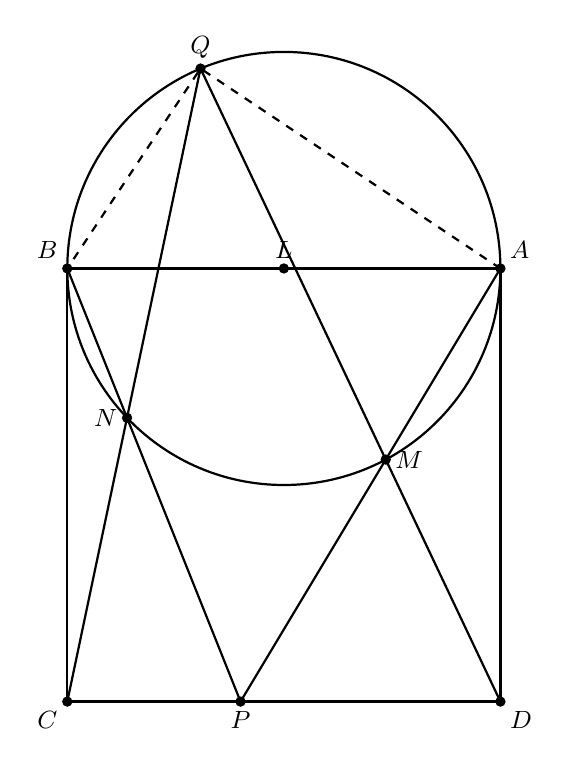
\begin{tikzpicture}[font=\small, scale=1.1]
    % Square ABCD: rotated so AB is top
    \coordinate[label=above right:$A$] (A) at (5,5);
    \coordinate[label=above left:$B$] (B) at (0,5);
    \coordinate[label=below left:$C$] (C) at (0,0);
    \coordinate[label=below right:$D$] (D) at (5,0);

    % Circle K with diameter AB, center L at midpoint of AB
    \coordinate[label=above:$L$] (L) at (2.5,5);
    \draw[thick] (L) circle (2.5);

    % Point P on CD, P = (2, 0)
    \coordinate[label=below:$P$] (P) at (2,0);

    % M = second intersection of AP with K
    \coordinate[label=right:$M$] (M) at (3.676, 2.794);

    % N = second intersection of BP with K
    \coordinate[label=left:$N$] (N) at (0.690, 3.276);

    % Q = DM \cap CN
    \coordinate[label=above:$Q$] (Q) at (1.538, 7.308);

    % Draw the square
    \draw[thick] (A)--(B)--(C)--(D)--cycle;

    % Draw lines AP and BP
    \draw[thick] (A)--(P);
    \draw[thick] (B)--(P);

    % Draw lines DM and CN (extended to Q)
    \draw[thick] (D)--(Q);
    \draw[thick] (C)--(Q);

    % Draw AQ and BQ to show angle AQB
    \draw[thick, dashed] (A)--(Q)--(B);

    % Mark right angles at M and N (angle in semicircle)
    \siku{A}{M}{B}
    \siku{A}{N}{B}
    \siku{A}{Q}{B}

    % Draw all points
    \foreach \s in {A,B,C,D,P,M,N,Q,L}
        \filldraw (\s) circle (1.5pt);
\end{tikzpicture}
\end{center}
Karena $K$ adalah lingkaran dengan diameter $AB$, maka $\angle AMB = \angle ANB = 90^\circ$. Untuk membuktikan $Q$ terletak pada $K$, cukup ditunjukkan $\angle AQB = 90^\circ$, atau $Q$ memenuhi persamaan lingkaran $K$.

Tanpa mengurangi keumuman, misalkan persegi \textbf{satuan} $ABCD$
\[A=(0,1),\quad B=(0,0), \quad C=(1,0), \quad D=(1,1).\]

Lingkaran $K$ berpusat di $L=\left(0,\tfrac{1}{2}\right)$ dengan jari-jari $\tfrac{1}{2}$, sehingga
\[x^2+\left(y-\tfrac{1}{2}\right)^2=\tfrac{1}{4}.\]

Misalkan $P=(1,t)$ untuk suatu $0\le t\le 1$.

Garis $AP$ dapat diparametrisasi menjadi $(s, 1-(1-t)s)$ untuk $s\ge 0$. Substitusi ke persamaan lingkaran $K$:
\begin{align*}
    s^2 + \left(\tfrac{1}{2}-(1-t)s\right)^2 &= \tfrac{1}{4}\\
    s\left((1+(1-t)^2)s - (1-t)\right) &= 0.
\end{align*}
Misalkan $u = 1-t$. Selain $s=0$ (titik $A$), didapat $s = \frac{u}{1+u^2}$, sehingga
\[M = \left(\frac{u}{1+u^2},\; \frac{1}{1+u^2}\right).\]

Lalu garis $BP$ dapat diparametrisasi sebagai $(s, ts)$ untuk $s\ge 0$. Substitusi ke persamaan lingkaran:
\begin{align*}
    s^2 + \left(ts-\tfrac{1}{2}\right)^2 &= \tfrac{1}{4}\\
    s\left((1+t^2)s - t\right) &= 0.
\end{align*}
Selain $s=0$ (yaitu titik $B$), didapat $s = \frac{t}{1+t^2}$, sehingga
\[N = \left(\frac{t}{1+t^2},\; \frac{t^2}{1+t^2}\right).\]

Sekarang, garis $DM$ dari $D=(1,1)$ dengan arah $(u^2-u+1,\; u^2)$ memiliki persamaan
\[u^2(x-1) = (u^2-u+1)(y-1).\]

Garis $CN$ dari $C=(1,0)$ dengan arah $(-(1-t+t^2),\; t^2)$ memiliki persamaan
\[t^2(x-1) = -(t^2-t+1)\,y.\]

Dari garis $CN$: $x = 1 - \frac{(t^2-t+1)}{t^2}\,y$. Substitusi ke garis $DM$ dan menggunakan $u^2-u+1 = t^2-t+1$:
\[\frac{-(1-t)^2}{t^2}\,y = y-1 \implies y = \frac{t^2}{t^2+(1-t)^2} = \frac{t^2}{2t^2-2t+1}.\]

Sehingga
\[x_Q = \frac{t(t-1)}{2t^2-2t+1}, \qquad y_Q = \frac{t^2}{2t^2-2t+1}.\]

Sekarang mari mengecek apakah $Q$ terletak pada lingkaran $K$:
\begin{align*}
    x_Q^2 + \left(y_Q - \tfrac{1}{2}\right)^2 
    &= \frac{t^2(t-1)^2}{(2t^2-2t+1)^2} + \left(\frac{2t^2 - (2t^2-2t+1)}{2(2t^2-2t+1)}\right)^2\\
    &= \frac{t^2(t-1)^2}{(2t^2-2t+1)^2} + \frac{(2t-1)^2}{4(2t^2-2t+1)^2}\\
    &= \frac{4t^2(t-1)^2 + (2t-1)^2}{4(2t^2-2t+1)^2}\\
    &= \frac{4t^4-8t^3+8t^2-4t+1}{4(2t^2-2t+1)^2}\\
    &= \frac{(2t^2-2t+1)^2}{4(2t^2-2t+1)^2} = \frac{1}{4}. \qquad \blacksquare
\end{align*}
Ternyata benar, damn.



\end{document}
